\documentclass[11pt,letterpaper]{article}

% --- Fonts and encoding ---
\usepackage[T1]{fontenc}
\usepackage{mathpazo}          % Palatino (consistent with other Theseus docs)
\usepackage{microtype}

% --- Page geometry ---
\usepackage[margin=1in]{geometry}

% --- Math ---
\usepackage{amsmath,amssymb,amsthm,mathtools}

% --- Graphics and diagrams ---
\usepackage{tikz}
\usetikzlibrary{arrows.meta,positioning,calc,decorations.pathmorphing,shapes.geometric,backgrounds,fit}

% --- Colors ---
\definecolor{accent}{HTML}{2E4057}
\definecolor{lightbg}{HTML}{F0F2F5}
\definecolor{midgray}{HTML}{6B7280}
\definecolor{deepred}{HTML}{9B2335}
\definecolor{deepblue}{HTML}{1E3A5F}
\definecolor{teal}{HTML}{0D7377}
\definecolor{amber}{HTML}{B8860B}
\definecolor{muted}{HTML}{8B8B8B}
\definecolor{softblue}{HTML}{D6E4F0}
\definecolor{softred}{HTML}{F0D6D6}
\definecolor{softgreen}{HTML}{D6F0D6}
\definecolor{softyellow}{HTML}{F5F0D0}
\definecolor{softpurple}{HTML}{E8D6F0}

% --- Section formatting ---
\usepackage{titlesec}
\titleformat{\section}{\large\bfseries\color{accent}}{\thesection}{1em}{}
\titleformat{\subsection}{\normalsize\bfseries\color{accent}}{\thesubsection}{1em}{}
\titleformat{\subsubsection}{\small\bfseries\color{accent}}{\thesubsubsection}{1em}{}

% --- Headers/footers ---
\usepackage{fancyhdr}
\pagestyle{fancy}
\fancyhf{}
\fancyhead[L]{\footnotesize\textsc{\color{midgray}Theseus Research}}
\fancyhead[R]{\footnotesize\textsc{\color{midgray}The Geometry of Unresolution}}
\fancyfoot[C]{\footnotesize\thepage}
\renewcommand{\headrulewidth}{0.4pt}

% --- Hyperlinks ---
\usepackage[colorlinks=true,linkcolor=accent,citecolor=accent,urlcolor=teal]{hyperref}

% --- Theorem environments ---
\theoremstyle{definition}
\newtheorem{definition}{Definition}[section]
\newtheorem{proposition}{Proposition}[section]
\newtheorem{theorem}{Theorem}[section]
\newtheorem{example}{Example}[section]
\theoremstyle{remark}
\newtheorem{remark}{Remark}[section]

% --- Insight boxes ---
\newenvironment{insightbox}{%
  \vspace{0.3cm}%
  \noindent\begin{tabular}{|p{\dimexpr\textwidth-4\tabcolsep-2\arrayrulewidth}|}
  \hline
  \small\itshape\color{accent}
}{%
  \\ \hline
  \end{tabular}
  \vspace{0.3cm}
}

% --- Epigraph ---
\usepackage{epigraph}
\setlength{\epigraphwidth}{0.75\textwidth}

\setlength{\parskip}{4pt plus 1pt minus 1pt}
\setlength{\parindent}{0pt}

% ====================================================================
\begin{document}

\thispagestyle{empty}

\vspace*{1.5cm}

\begin{center}
{\Large\bfseries\color{accent} The Geometry of Unresolution}\\[8pt]
{\large\color{midgray} Mathematical Frameworks for Modelling\\[2pt] Incomplete Epistemic States}\\[20pt]
{\normalsize Theseus Research Division}\\[4pt]
{\footnotesize\color{muted} April 2026}
\end{center}

\vspace{0.5cm}

\epigraph{\itshape The opposite of a correct statement is a false statement. But the opposite of a profound truth may well be another profound truth.}{--- Niels Bohr}

\vspace{0.3cm}

\begin{abstract}
\noindent
Imagine you and a colleague have spent months building a shared understanding of a difficult question. You've uncovered many truths, refuted some initial hypotheses, and converged on what feels like solid ground. Yet when you map your actual beliefs, you discover something unsettling: your conclusions are subtly contradictory, or you've been using the same words to mean different things, or your frameworks are incompatible in ways that only become visible from a certain angle. This is the phenomenon of \emph{unresolution}: the existence of genuine insight alongside genuine contradiction, with no clear boundary between them.

This paper surveys twelve mathematical frameworks---drawn from algebraic topology, lattice theory, paraconsistent logic, information geometry, and category theory---that give rigorous geometric and algebraic characterisations of states of partial resolution. We identify five cross-cutting structural motifs (boundary as signature, multi-scale filtration, lattice order, cohomological obstruction, convexity of imprecision) and propose that unresolution is not a deficiency to be eliminated but a geometrically structured feature of any living epistemic system. The analysis yields concrete diagnostics for the Noosphere coherence engine: persistent homology detects the \emph{scale} at which ideas resist synthesis; sheaf cohomology localises \emph{where} global consistency fails; and the Fisher information metric measures how \emph{far} one stands from resolution in the space of credal states.
\end{abstract}

\vspace{0.4cm}
\hrule
\vspace{0.4cm}
\tableofcontents
\vspace{0.4cm}
\hrule

\newpage

% ====================================================================
\section{A Reader's Guide: Why This Matters}

This document is written for people who care about making sense of complex, evolving knowledge---whether you're building a research system, managing a team, or trying to understand why smart people disagree. You don't need to know topology or category theory.

\subsection*{The Core Insight}

When you track a group of ideas over time, three things typically happen:

First, they resolve: what seemed contradictory turns out to be compatible once you understand the context. Or one position convinces everyone and the alternative fades. This is what we're used to calling ``progress''.

Second, they crystallise into genuine contradiction: the evidence clearly rules one out. This is resolution through negation.

But there's a third possibility, and it's where this paper focuses: ideas can coexist without being resolved into either harmony or contradiction. They resist synthesis without being refutable. This happens constantly in science, philosophy, and organisational decision-making, and when it does, we need a language for it.

This paper gives you that language. It shows that unresolution is not featureless ignorance. It has shape. It has layers. It has patterns you can measure. Some unresolved tensions are superficial---they dissolve if you look at the problem from a slightly different angle. Others are structural---no amount of evidence or reframing will resolve them within the current framework. Knowing the difference is powerful.

\subsection*{What You'll Find Here}

We survey twelve mathematical frameworks, each offering a different lens on unresolution:

\textbf{Topological frameworks} (persistent homology, topological epistemic logic) ask: what is the \emph{shape} of unresolution? Do contradictions cluster at one scale or many? What does the landscape of tension look like?

\textbf{Algebraic frameworks} (sheaf theory, rough sets, lattices) ask: where is unresolution \emph{located}? Is it global or local? Can it be decomposed?

\textbf{Logical frameworks} (paraconsistent logic, quantum logic) ask: what are the \emph{types} of unresolution? Is something unresolved because we lack information, or because we have contradictory information, or because our frameworks are incommensurable?

\textbf{Information-geometric frameworks} (Dempster--Shafer, Fisher information) ask: how \emph{far} are we from resolution? Can we measure it? What would it take to cross the boundary?

\subsection*{For Practitioners}

If you're building a system like Noosphere, or trying to diagnose why a team's reasoning has stalled:

\begin{itemize}
\item Use \textbf{persistent homology} (Section~\ref{sec:persistent}) to find which tensions are structural and which are noise.
\item Use \textbf{sheaf cohomology} (Section~\ref{sec:sheaf}) to find which pairs of topics are pulling in opposite directions.
\item Use \textbf{paraconsistent logic} (Section~\ref{sec:paraconsistent}) to distinguish between ``we haven't investigated enough'' and ``we have genuine contradiction.''
\item Use the \textbf{decision guide} (Section~\ref{sec:decision}) to pick the right diagnostic for your situation.
\end{itemize}

\subsection*{Organisation}

Sections~\ref{sec:topological}--\ref{sec:categorical} survey the frameworks. Each subsection includes a plain-language analogy, a worked example, mathematical definitions, and a ``what this tells us'' box. Sections~\ref{sec:motifs} and~\ref{sec:hierarchy} show how they fit together. Section~\ref{sec:history} traces the intellectual origins. Section~\ref{sec:computational} discusses algorithmic complexity. Section~\ref{sec:taxonomy} proposes a unified classification of unresolution types. Section~\ref{sec:limitations} addresses what these frameworks cannot do. Section~\ref{sec:noosphere} shows how to implement them. Section~\ref{sec:decision} provides a decision flowchart. Section~\ref{sec:conclusion} synthesises the findings.

\vspace{0.3cm}

You can read this linearly, or skip to the section that matches your current problem. The frameworks are independent enough that reading them in any order makes sense.

\newpage

% ====================================================================
\section{Historical Context: How We Got Here}
\label{sec:history}

The question ``what is the structure of unresolution?'' has haunted mathematics and philosophy for centuries. This section traces that intellectual genealogy.

\subsection{Ancient and Medieval Foundations}

Aristotle formulated the law of excluded middle: every proposition is either true or false, and there is no middle ground. This became the foundation of classical logic, and it worked remarkably well---until it didn't. In his sea-battle argument, Aristotle himself noted a problem: \emph{The naval battle tomorrow}: is the statement ``it will happen'' true or false today? If true today, the future is predetermined; if false, the future is predetermined in the opposite direction. Yet we experience the future as genuinely open. The statement resists bivalence---it is genuinely unresolved, not out of ignorance, but out of the structure of time.

Medieval logicians (Aquinas, Scotus, William of Ockham) grappled with divine omniscience and human free will: how can God know all futures if those futures are genuinely open? The solutions ranged from denying human freedom to proposing that God experiences time differently. But the core issue remained: some statements are unresolved in a way that is not merely epistemic (ignorance) but metaphysical (structure of reality).

\subsection{19th-Century Mathematics and Logic}

Georg Cantor's work on infinite sets revealed that some questions cannot be answered within a given mathematical framework. The continuum hypothesis cannot be proven or disproven from the axioms of set theory---it is unresolved structurally, not just epistemically. This was shocking.

\subsection{Gödel, Tarski, and Incompleteness (1930s)}

Kurt Gödel's incompleteness theorems (1931) made this concrete: every consistent formal system strong enough to express arithmetic contains true statements that are unprovable within the system. Unresolution is not a bug in our formal systems; it is a fundamental feature of how formal systems work. Some questions are structurally unresolvable: they cannot be answered from within the system, even in principle.

Alfred Tarski's work on truth (1933) showed that truth itself cannot be axiomatised without contradiction. The attempt to create a self-referential theory of truth generates paradoxes (the liar's paradox). This is another form of structural unresolution: the very act of trying to resolve the question generates contradiction.

\subsection{Quantum Mechanics and Superposition (1920s--1930s)}

Quantum mechanics introduced a different kind of unresolution: superposition. An electron is not simultaneously in two places and also something else; rather, it is in a state that cannot be decomposed into classical possibilities. Niels Bohr articulated the complementarity principle: certain pairs of properties (position and momentum, energy and time) are mutually exclusive in the sense that measuring one makes the other indeterminate. The system is unresolved not because we lack information, but because the very notion of ``the value is precisely this'' is inapplicable.

John von Neumann and Garrett Birkhoff showed that the lattice of quantum propositions is not Boolean---it is orthomodular, which means distributivity fails. This non-distributivity is the formal expression of superposition. The geometry of unresolution in quantum mechanics is the geometry of a non-Boolean lattice.

\subsection{Intuitionism and Constructivism (1920s--1930s)}

L.E.J. Brouwer's intuitionism rejected the law of excluded middle. For a constructivist, a statement is only meaningful if there is an effective procedure (a proof) for establishing it. Many statements lack such procedures, and for the intuitionist, these are not merely epistemically unresolved---they are indeterminate in principle. Brouwer believed that mathematical truth is a matter of mental construction, not discovery, and that many classical theorems rest on invalid reasoning.

The implications were radical: classical logic is not the foundation of mathematics; it is one possible framework among many. Other logics---intuitionistic logic, linear logic, affine logic---reveal different structures of validity and invalidity. Unresolution, on this view, is not a defect in our system but a sign that we are trying to force classical logic onto a problem that requires a different framework.

\subsection{Fuzzy Logic and Many-Valued Logic (1960s--1970s)}

Lotfi Zadeh's fuzzy logic (1965) rejected bivalence in a different way. Instead of propositions being true or false, truth became a continuous function: a proposition is true to degree $0.7$, false to degree $0.4$, etc. This turned unresolution into gradation: a proposition can be partially true and partially false. The boundaries between categories are not sharp lines but continuous transitions.

\c{S}ve Fej\'er and others developed many-valued logics: instead of $\{T, F\}$, we have $\{T, F, U\}$ (unknown), or four values, or infinitely many. The Belnap--Dunn four-valued logic (1970s) was particularly influential: it distinguished between ignorance ($\bot$: neither true nor false) and contradiction ($\top$: both true and false). This distinction is mathematically precise and operationally meaningful.

\subsection{Category Theory and Universal Properties (1940s--1970s)}

Samuel Eilenberg and Saunders Mac Lane's category theory (1945) provided a language for talking about ``incompleteness'' in a new way. In a category, a limit of a diagram need not exist. The non-existence of a limit is not a deficiency; it is a structural fact about how the diagram sits in the category. If you want to force the limit to exist, you must change the category.

This reframed the question: unresolution is not about our knowledge; it is about the structure of the space of possibilities. Some things are unresolvable \emph{in this category}, but might be resolvable in a larger category. The choice of category is a choice of framework, and unresolution depends on that choice.

\subsection{Persistence and Topological Data Analysis (2000s)}

Gunnar Carlsson and Afra Zomorodian developed persistent homology (2000s), combining ideas from algebraic topology with computational data analysis. This provided a concrete method for detecting topological features that persist across scales. For the first time, we had an algorithm for finding the ``robust'' features in a dataset, the ones that remain as parameters vary.

The key insight for unresolution: topological features that survive perturbation are structurally significant, while features that vanish are noise. Unresolution that persists across many scales is real; unresolution that vanishes when you look more carefully is superficial.

\subsection{Higher Type Theory and HoTT (2000s--2010s)}

Homotopy type theory, developed in the 2000s--2010s by Vladimir Voevodsky, Martin Hofmann, Thomas Streicher, Benedikt Ahrens, and others, introduced a new way to think about identity. In HoTT, the identity type between two objects is not merely a proposition (true or false) but a space whose topology encodes the different ways those objects can be identified.

This provided a framework for thinking about higher-order unresolution: not just whether two things are the same, but how many ways there are for them to be the same, and what the relationship is between those ways.

\subsection{Synthesis}

The common thread across these developments: unresolution is not a superficial phenomenon (ignorance that will fade with more information) but a deep feature of how knowledge works. It manifests differently in different domains (semantics, quantum mechanics, intuitionism, topology), but it is always present. And in each domain, it has geometric structure.

This paper brings these frameworks together under one roof.

\newpage

% ====================================================================
\section{Topological Approaches}
\label{sec:topological}

\subsection{Persistent Homology: Unresolution as Multi-Scale Topology}
\label{sec:persistent}

\subsubsection*{Plain-Language Analogy}

Imagine a landscape of mountains and valleys representing claims and tensions between them. If you raise a ``fog level'' and watch which valleys become isolated islands, you see which mountain ranges are truly separate. Some islands appear early (at low fog) because the peaks are far apart; others appear late because the valleys between them are deep. As the fog rises further, islands merge back together: first the close neighbors, then the distant ones. Which islands persist for the longest range of fog levels? Those are the truly significant features of the landscape. Temporary islands that quickly merge are noise. Persistent islands are signal. This is what persistent homology does with epistemic claims.

\subsubsection*{Worked Example: Wave-Particle Duality}

Consider the historical debate over whether light is a wave or a particle. In the 17th century, Newton argued for particles; Huygens argued for waves. By the late 19th century, Maxwell's equations suggested waves; the photoelectric effect suggested particles. In 1905--1927, quantum mechanics emerged as a framework where light is \emph{neither} in the classical sense, but described by a wave function $\psi$ that gives probabilities for particle-like observations.

Build a claim graph with two clusters: $(C_{\text{wave}}) = \{\text{claims supporting wave picture}\}$ and $(C_{\text{particle}}) = \{\text{claims supporting particle picture}\}$. Embed these as vectors in a high-dimensional space. Compute a Vietoris--Rips filtration: at distance $\epsilon_1$, the two clusters are separate; as $\epsilon$ increases, they begin to touch; at $\epsilon_2$, they merge into one connected component.

Now compute $H_1$ (loops): at some distance $\epsilon_*$, a loop is born that connects claims from both clusters in a cycle. This loop represents a dialectical tension: claim $W$ from the wave picture implies claim $P_1$, which contradicts claim $P_2$ from the particle picture, which implies claim $P_3$, which contradicts claim $W'$ (a variant of $W$), and so on. The loop persists (does not collapse) because the tension is structural.

The persistence diagram shows: $H_0$ (components) has short lifetime (clusters merge quickly, suggesting the distinction is superficial). $H_1$ (loops) has long lifetime, stretching from early $\epsilon$ to late $\epsilon$, suggesting the tension is robust across many scales of analysis. The conclusion: wave-particle duality is not merely a surface-level confusion; it reflects a deep topological incommensurability in how we model reality.

\subsubsection*{Mathematical Details}

\begin{definition}[Persistence Module]
Given a filtered simplicial complex $\{K_\epsilon\}_{\epsilon \geq 0}$ built on a set of epistemic claims (e.g., a Vietoris--Rips complex on embedding vectors), a \textbf{persistence module} is the sequence of homology groups
\[
H_k(K_{\epsilon_0}) \to H_k(K_{\epsilon_1}) \to H_k(K_{\epsilon_2}) \to \cdots
\]
induced by the inclusion maps $K_{\epsilon_i} \hookrightarrow K_{\epsilon_j}$ for $\epsilon_i \leq \epsilon_j$.
\end{definition}

A feature (generator of $H_k$) is \textbf{born} at scale $\epsilon_b$ when it first appears in some $H_k(K_{\epsilon_b})$ and is not in the image of the map from $H_k(K_{\epsilon_b - \delta})$. It \textbf{dies} at scale $\epsilon_d$ when it is killed by the boundary map to $H_{k-1}(K_{\epsilon_d})$. The pair $(\epsilon_b, \epsilon_d)$ is recorded as a point in the \textbf{persistence diagram} $\mathrm{Dgm}_k$.

\begin{proposition}[Stability]
(Bottleneck Stability Theorem) Let $\mathrm{Dgm}_k(\mathcal{C})$ and $\mathrm{Dgm}_k(\mathcal{C}')$ be persistence diagrams from two claim clusters that differ by Hausdorff distance $\delta$ (in embedding space). Then the bottleneck distance between the diagrams is at most $\delta$:
\[
d_B(\mathrm{Dgm}_k(\mathcal{C}), \mathrm{Dgm}_k(\mathcal{C}')) \leq \delta.
\]
This means small perturbations in embeddings produce small perturbations in the diagram. The geometry of unresolution is robust.
\end{proposition}

\subsubsection*{Computational Complexity}

Computing persistence diagrams is $O(n^3)$ in the worst case (using discrete Morse theory), but modern algorithms (e.g., PHAT, Ripser) achieve $O(n^2 \log n)$ for Vietoris--Rips complexes in practice. For a claim graph with $n = 10{,}000$ claims, this is computationally feasible on standard hardware.

\begin{insightbox}
\textbf{What This Tells Us:} A long-lived feature in a persistence diagram signals that claims are not merely locally inconsistent but form cycles of tension at many scales. This is the topological signature of irresolvable contradiction (in the Hegelian sense: a tension that drives deeper understanding). Conversely, short-lived features are ephemeral: they may disappear if you re-embed the claims or refine the distance metric. When choosing what tensions to invest effort in resolving, prioritise the long-lived ones.
\end{insightbox}

\subsection{Topological Epistemic Logic: Boundary as Ignorance}
\label{sec:topological-logic}

\subsubsection*{Analogy}

In a medieval city with walls and gates, the city interior is ``known territory'' (the closed set where knowledge is certain) and the countryside is ``uncertain territory'' (where knowledge is partial). The walls themselves---the boundary---are the zone of maximum uncertainty: from inside the walls you can see the farms and roads just beyond; from outside you see the city but cannot enter. The boundary is where your epistemic status is most ambiguous.

\subsubsection*{Mathematical Framework}

McKinsey and Tarski (1944) showed that modal logic S4 (the logic of necessity and possibility) is the logic of topological spaces. The interpretation is:

\begin{itemize}
\item $\mathrm{Int}(A)$ (interior of $A$): the set of points where $A$ is certainly true.
\item $\mathrm{Cl}(A)$ (closure of $A$): the set of points where $A$ is possibly true (or cannot be ruled out).
\item $\partial A = \mathrm{Cl}(A) \setminus \mathrm{Int}(A)$ (boundary): the set where $A$ is neither certain nor impossible.
\end{itemize}

\begin{proposition}[Topological Characterisation]
A proposition $A$ is fully resolved if $\partial A = \emptyset$ (the boundary is empty: the truth value is known everywhere). The proposition is deeply unresolved if $\partial A$ is thick and complex. The dimension of the boundary (as a topological manifold) characterises the \emph{depth} of unresolution.
\end{proposition}

\begin{theorem}[Boundary Structure]
In a topological space, the boundary of any set is always closed and nowhere dense. This means unresolved regions are always ``thin''---they have measure zero and are nowhere in the interior of the unresolved region. Topologically, resolution is the default and unresolution is exceptional.
\end{theorem}

\subsubsection*{Worked Example: Realism vs.\ Anti-Realism in Science}

The debate between realists (scientific theories describe reality as it is) and anti-realists (theories are useful instruments but do not describe reality) cannot be resolved by empirical observation alone. Every empirical datum is consistent with both interpretations. The boundary $\partial A$ (where $A$ = ``the theory is realist'') includes every conceivable epistemic state: we can be fully convinced of the correctness of the theory and still uncertain about whether it is realist. This boundary is not merely thick; it is \emph{thick everywhere} (the interior is empty, the closure is everything). The debate is not resolvable within empiricist frameworks.

\subsubsection*{Computational Complexity}

Deciding whether $\partial A = \emptyset$ for a finite epistemic state is NP-complete (it requires checking all possible consistent assignments). For practical epistemic systems, approximations are necessary: sample the belief space and estimate the fraction of points where $A$ is undetermined.

\begin{insightbox}
\textbf{What This Tells Us:} If a question has a thick, complex boundary, it is unresolvable through empirical investigation alone. It requires a shift in framework (a topological ``folding'' of the space) to gain resolution. Questions with thin boundaries can be resolved by gathering more evidence. Questions with thick boundaries require conceptual innovation.
\end{insightbox}

\newpage

% ====================================================================
\section{Algebraic and Lattice-Theoretic Approaches}
\label{sec:algebraic}

\subsection{Sheaf Cohomology: Local Consistency, Global Failure}
\label{sec:sheaf}

\subsubsection*{Analogy}

Imagine a city where each neighborhood has its own interpretation of the law: in the North District, property law is interpreted one way; in the South District, another way. Within each neighborhood, the interpretation is consistent. But when you look at the boundaries between neighborhoods, you find contradictions: a property that is ``rightfully owned'' under North District law is ``rightfully seized'' under South District law. When you try to ask ``who owns the property?'' globally, you run into a problem that cannot be solved by adjusting the interpretation in any single district. You need a global law that harmonises all local interpretations. If no such global law exists, the city is globally incoherent despite local coherence. Sheaf cohomology detects exactly this: where global coherence fails despite local coherence.

\subsubsection*{Mathematical Framework}

\begin{definition}[Presheaf of Epistemic States]
Let $\mathcal{U} = \{U_i\}$ be an open cover of an epistemic space (e.g., topic clusters in the claim graph). A \textbf{presheaf} $\mathcal{F}$ assigns to each open set $U_i$ a set of locally consistent interpretations $\mathcal{F}(U_i)$, with restriction maps $\rho_{ij}: \mathcal{F}(U_i) \to \mathcal{F}(U_i \cap U_j)$ expressing compatibility on overlaps.
\end{definition}

$\mathcal{F}$ is a \textbf{sheaf} if and only if:
\begin{enumerate}
\item Local sections that agree on overlaps can be uniquely glued: if $s_i \in \mathcal{F}(U_i)$ and $s_j \in \mathcal{F}(U_j)$ with $\rho_{ij}(s_i) = \rho_{ji}(s_j)$ on overlaps, then there exists a unique global section $s \in \mathcal{F}(\bigcup U_i)$ restricting to $s_i$ on each $U_i$.
\end{enumerate}

\begin{proposition}[Cohomological Signature of Unresolution]
If $\mathcal{F}$ fails the gluing condition (local coherence cannot be extended to global coherence), the \textbf{first Čech cohomology} $H^1_{\check{\mathrm{C}}}(\mathcal{U}, \mathcal{F})$ is non-trivial. Each non-zero cohomology class $[\omega] \in H^1(\mathcal{U}, \mathcal{F})$ represents an \emph{irreducible mode of unresolution}---a pattern of local-global inconsistency that cannot be eliminated by adjusting any single local interpretation.
\end{proposition}

\subsubsection*{Worked Example: Free Will vs.\ Determinism}

Consider a debate with multiple subtopics: physics (deterministic or indeterministic laws), neuroscience (brain processes as physical systems), and ethics (responsibility requires freedom). Within each subtopic, there are coherent positions: physicists can defend determinism, neuroscientists can defend physicalism, ethicists can defend compatibilism (free will is compatible with determinism). Each position is internally consistent.

But when you try to harmonise them globally, you run into tension. A globally coherent system must either:
\begin{itemize}
\item Accept indeterminism (physics) to preserve libertarian free will (ethics).
\item Accept determinism (physics) and compatibilism (ethics) to preserve physicalism (neuroscience).
\item Or introduce some other framework-level shift (e.g., epiphenomenalism: consciousness is causally inert).
\end{itemize}

Each global choice sacrifices some local coherence. The non-vanishing of $H^1$ signals that no choice is fully satisfactory; every option requires compromising some local consensus.

\subsubsection*{Computational Complexity}

Computing Čech cohomology from a finite open cover requires:
\begin{enumerate}
\item Representing each local coherence set as a polytope (or other convex structure).
\item Computing intersection polytopes for all pairwise and higher-order overlaps: $O(2^{|\mathcal{U}|})$ intersections in the worst case.
\item Solving a system of linear constraints to find the kernel and image of the coboundary maps: $O(n^3)$ per layer.
\end{enumerate}

For $|\mathcal{U}| = 8$ topics, this is computationally feasible. For $|\mathcal{U}| = 20+$, approximations are necessary (e.g., sample-based cohomology).

\begin{insightbox}
\textbf{What This Tells Us:} Non-zero cohomology is not a defect; it is information. It tells you that the system harbours an unresolvable tension at the \emph{inter-topic level}. Trying to resolve it by adjusting claims within a single topic will fail. You need cross-topic synthesis or framework innovation. The dimension of $H^1$ counts the independent degrees of freedom of this inter-topic irresolution.
\end{insightbox}

\subsection{Rough Set Theory: The Boundary Region}

\subsubsection*{Analogy}

A doctor examining a patient with partial information (symptoms, but not all tests) cannot definitively diagnose a disease; instead, she marks some patients as ``certainly in the disease category'' (they show all definitive symptoms) and some as ``possibly in the disease category'' (they show some symptoms, but the diagnosis is uncertain). The patients in between are the ``boundary''---those whose status is undetermined by available distinctions. As the doctor gathers more information (more tests, finer distinctions), the boundary shrinks. The rate at which it shrinks measures the ``difficulty'' of the diagnostic problem.

\subsubsection*{Mathematical Framework}

Pawlak's rough set theory (1982) formalises this. Given an indiscernibility relation $R$ (an equivalence relation expressing ``indistinguishable given current information''), and a target concept $X$:

\[
\underline{R}(X) = \{x \in U : [x]_R \subseteq X\}, \quad \overline{R}(X) = \{x \in U : [x]_R \cap X \neq \emptyset\}
\]

where $[x]_R$ is the equivalence class of $x$ under $R$. The \textbf{boundary region} is:
\[
\mathrm{BN}_R(X) = \overline{R}(X) \setminus \underline{R}(X).
\]

The \textbf{roughness index} is:
\[
\rho_R(X) = 1 - \frac{|\underline{R}(X)|}{|\overline{R}(X)|}.
\]

\begin{example}[Epistemic Applications]
Suppose $X$ = ``the claim is true,'' $R$ = ``indistinguishability given current evidence,'' and the universe $U$ = ``all possible claims.''
\begin{itemize}
\item $\underline{R}(X)$: claims for which the current evidence proves truth.
\item $\overline{R}(X)$: claims that the evidence permits (does not rule out).
\item $\mathrm{BN}_R(X)$: claims in genuine epistemic limbo (some evidence supports, some permits but does not require).
\item $\rho_R(X)$ near 0: claim is nearly fully resolved (small boundary).
\item $\rho_R(X)$ near 1: claim is nearly fully unresolved (large boundary).
\end{itemize}
\end{example}

\subsubsection*{Computational Complexity}

Computing rough approximations given an indiscernibility relation requires partitioning the universe (finding equivalence classes): $O(n \log n)$ with sorting. Computing roughness for all concepts: $O(n \cdot |X|)$. Refining the relation (adding finer distinctions) requires recomputing from scratch.

\begin{insightbox}
\textbf{What This Tells Us:} A high roughness index means the question is difficult---not because we lack intelligence, but because available distinctions are insufficient. Resolving it requires new concepts, new measurements, or new information sources. A low roughness index means the question is tractable with current tools. This gives a concrete way to prioritise research efforts.
\end{insightbox}

\subsection{Formal Concept Analysis: The Lattice of Partial Understanding}
\label{sec:fca}

\subsubsection*{Analogy}

Imagine a library where you can browse books by subject (attribute space) and readers come in looking for knowledge (object space). Some combinations are common: ``logic books by philosophers''; others are rare: ``logic books by novelists.'' The lattice of concepts organises all possible combinations into a hierarchy: the most general concept (all books) sits at the top; the most specific concepts (a single book by a single attribute) sit at the bottom. If you find a huge antichain in the middle (many concepts that are incomparable---neither more general nor more specific), it means there are many distinct ways of organising the knowledge, and no single hierarchy captures it all. This incomparability is a sign of conceptual pluralism.

\subsubsection*{Mathematical Framework}

In Formal Concept Analysis (FCA), a \textbf{formal context} is $(G, M, I)$ where $G$ is a set of objects, $M$ is a set of attributes, and $I \subseteq G \times M$ is the incidence relation (which objects have which attributes). A \textbf{formal concept} is a pair $(A, B)$ where $A \subseteq G$ and $B \subseteq M$ are \emph{closed} under the derivation operators:

\[
A' = \{m \in M : (g, m) \in I \text{ for all } g \in A\}, \quad B' = \{g \in G : (g, m) \in I \text{ for all } m \in B\}.
\]

The concept lattice $\mathfrak{B}(G, M, I)$ orders concepts by extent: $(A_1, B_1) \leq (A_2, B_2)$ iff $A_1 \supseteq A_2$ (and equivalently $B_1 \subseteq B_2$).

\subsubsection*{Epistemological Interpretation}

In FCA, unresolution manifests as:
\begin{itemize}
\item \textbf{Width}: the maximum antichain size (number of mutually incomparable concepts). A wide lattice has many concepts that do not fit into a linear hierarchy. This signals conceptual pluralism.
\item \textbf{Height}: the longest chain from bottom to top. A tall lattice has deep subsumption hierarchies.
\item \textbf{Partial concepts}: pairs of sets $(A, B)$ that are not closed under derivation, representing ideas that are neither entailed nor excluded.
\end{itemize}

\begin{proposition}[Incomparability as Unresolution]
If the concept lattice has a large antichain $\{(A_i, B_i) : i = 1, \ldots, k\}$, then there are $k$ essentially different ways of organising the objects and attributes. These are not ordered by generality/specificity, so no single conceptual hierarchy captures all of them. This is a sign of irreducible conceptual unresolution.
\end{proposition}

\subsubsection*{Computational Complexity}

Computing the full concept lattice from a context is NP-hard (the lattice can have exponentially many concepts). However, for practical purposes, one can compute the lattice incrementally or sample it.

\begin{insightbox}
\textbf{What This Tells Us:} A wide, incomparable lattice of concepts suggests that the domain has genuine structural diversity: it cannot be hierarchically organised without loss. Rather than forcing a single hierarchy (which always requires lossy projection), acknowledge the diversity and use pluralistic frameworks. The width of the antichain measures how much conceptual diversity the system contains.
\end{insightbox}

\newpage

% ====================================================================
\section{Logic-Based Approaches}
\label{sec:logic}

\subsection{Paraconsistent Logic: The Belnap--Dunn Bilattice}
\label{sec:paraconsistent}

\subsubsection*{Analogy}

In classical logic, contradiction makes everything provable (ex falso quodlibet): if you derive both $P$ and $\neg P$, you can prove any statement, true or false. It's as if the system explodes. But in real epistemic systems, contradictions do not cause explosion---they coexist with sensible reasoning. A paraconsistent logic is one where contradiction is tolerated: you can have both $P$ and $\neg P$ in the system without being able to prove that your grandmother is a teapot.

The Belnap--Dunn four-valued logic distinguishes four truth values: $\mathbf{t}$ (true), $\mathbf{f}$ (false), $\top$ (both true and false), and $\bot$ (neither). This distinction is not arbitrary; it cuts reality at a real joint.

\subsubsection*{Worked Example: Medical Uncertainty}

A patient tests positive for a disease, but the test has a false-positive rate. Should we say the patient has the disease ($\mathbf{t}$), does not have the disease ($\mathbf{f}$), or is the status uncertain ($\bot$)?

In classical logic, the answer is $\mathbf{t}$ or $\mathbf{f}$---there is no middle ground. In fuzzy logic, the answer is a number between 0 and 1: maybe 0.75 (seventy-five percent likely). But the Belnap--Dunn framework offers something different: the status is $\bot$ (neither $\mathbf{t}$ nor $\mathbf{f}$ in the strong sense) if we lack evidence. It is $\top$ if we have \emph{contradictory} evidence: both the test result (suggesting disease) and the absence of symptoms (suggesting no disease).

This distinction is operationally crucial:
\begin{itemize}
\item $\bot$ (ignorance) calls for \emph{more evidence}: we need a better test or more data.
\item $\top$ (contradiction) calls for \emph{conceptual revision}: maybe the disease manifests differently in some patients, or the test measures something other than what we thought.
\end{itemize}

Conflating them leads to wrong action.

\subsubsection*{Mathematical Framework}

The Belnap--Dunn bilattice has two partial orders:

\textbf{Truth order} ($\mathbf{t}$ and $\mathbf{f}$ are maximal):
\[
\mathbf{f} \leq \bot, \quad \mathbf{f} \leq \top, \quad \bot \leq \mathbf{t}, \quad \top \leq \mathbf{t}.
\]

\textbf{Knowledge order} ($\top$ and $\bot$ are extremal):
\[
\bot \leq \mathbf{t}, \quad \bot \leq \mathbf{f}, \quad \mathbf{t} \leq \top, \quad \mathbf{f} \leq \top.
\]

\begin{remark}[Operational Meaning]
The truth order says: $\mathbf{t}$ and $\mathbf{f}$ are the ``good'' states (fully determined); intermediate values are ``bad.'' The knowledge order says: $\top$ is the worst (we have conflicting signals) and $\bot$ is the best in the sense of being determined (we have clear consensus)---no, wait, that's wrong. $\top$ is the worst (contradictory information) and $\bot$ is best (though least informative). The confusion here is endemic to thinking about unresolution; the bilattice separates the two intuitions and makes them precise.
\end{remark}

\subsubsection*{Computational Complexity}

Evaluating a formula in Belnap--Dunn logic is polynomial in the size of the formula and the assignment (similar to classical logic). The challenge is in designing coherence procedures that detect and reconcile contradictions.

\begin{insightbox}
\textbf{What This Tells Us:} Before accepting a contradiction as genuine, ask: do we lack evidence ($\bot$), or do we have conflicting evidence ($\top$)? In the first case, investigate further. In the second case, something in the framework must change. A system that conflates ignorance and contradiction wastes effort investigating questions that are not resolvable through investigation.
\end{insightbox}

\subsection{Quantum Logic: Superposition as Structural Indeterminacy}

\subsubsection*{Analogy}

In classical logic, propositions are combined using AND, OR, and NOT. These operations have a simple structure: they follow Boolean algebra, which is distributive. But in quantum mechanics, the propositions (statements about physical systems) do not obey distributivity. This is not because we lack knowledge; it is because the logical structure of quantum propositions is fundamentally different from classical propositions.

Think of a proposal that depends on the context: ``do you approve of raising taxes?'' might receive ``yes'' if the money goes to education and ``no'' if it goes to military spending. The answer is not independent of context. In classical logic, there is no direct way to model this: you'd need to expand the propositions (``do you approve of raising taxes for education?'') and lose the sense of a single context-dependent judgment. Quantum logic allows propositions to be context-dependent, which is closer to how real epistemic agents work.

\subsubsection*{Mathematical Framework}

The lattice of closed subspaces of a Hilbert space is an \textbf{orthomodular lattice}: a partial order $(L, \leq)$ with meet $\wedge$, join $\vee$, and orthogonal complement $\perp$ satisfying:

\begin{enumerate}
\item \textbf{Distributivity fails}: $P \wedge (Q \vee R)$ need not equal $(P \wedge Q) \vee (P \wedge R)$.
\item \textbf{Orthomodular law}: if $P \perp Q$ then $P = (P \wedge Q) \vee (P \wedge Q^\perp)$.
\end{enumerate}

The failure of distributivity is the formal expression of superposition.

\subsubsection*{Epistemological Interpretation}

If epistemic claims form an orthomodular lattice (rather than Boolean), it means some pairs of claims are framework-dependent: the truth value of one depends on whether the other is asserted. This happens when paradigms are incommensurable or when the meaning of terms shifts contextually.

\begin{proposition}[Non-Distributivity as Framework-Dependence]
If $P \wedge (Q \vee R) \neq (P \wedge Q) \vee (P \wedge R)$, then there is no way to evaluate $P$, $Q$, and $R$ independently of each other. The truth value of $P$ depends on whether we evaluate in the context of $Q$ or $R$. This is the formal signature of framework-dependent claims.
\end{proposition}

\subsubsection*{Computational Complexity}

Evaluating formulas in quantum logic is also polynomial, but the challenge is in representing the lattice structure computationally (which requires specifying closure relationships and orthogonality).

\begin{insightbox}
\textbf{What This Tells Us:} Some tensions cannot be resolved by choosing a single interpretation because the claims are framework-dependent. Rather than asking ``is $P$ true?'' ask ``is $P$ true in framework $F$?'' The geometry of framework-dependence is the geometry of the non-Boolean lattice.
\end{insightbox}

\newpage

% ====================================================================
\section{Probabilistic and Information-Geometric Approaches}
\label{sec:probabilistic}

\subsection{Dempster--Shafer Theory: The Plausibility--Belief Gap}
\label{sec:ds}

\subsubsection*{Analogy}

Suppose you ask three experts whether a hypothesis is true. Expert A says: ``I'm 60\% confident it's true.'' Expert B says: ``The evidence points to truth with high likelihood, but I'm not fully convinced, so I'd say 70\%.'' Expert C says: ``I really can't decide; the evidence is mixed.''

In Bayesian probability, you'd average these (maybe 65\%) or use a weighted combination. But what if the experts are not providing probabilities? What if A is saying ``at least 60\% of the evidence supports truth,'' B is saying ``up to 70\% is consistent with truth,'' and C is saying ``the evidence is too mixed to narrow it down further''?

Then the true probability is somewhere in an interval: between 60\% and 70\% maybe, or even wider. Dempster--Shafer theory formalises this: instead of assigning probability to each hypothesis, you assign mass to \emph{sets} of hypotheses, and the belief and plausibility functions bracket the true probability.

\subsubsection*{Worked Example: Conspiracy Theories}

Consider a claim: ``The government is covering something up.'' Evidence includes:
\begin{itemize}
\item The government \emph{did} cover something up historically (plenty of examples).
\item But not every government claim is false.
\item Some people claim the cover-up without evidence.
\item But absence of evidence is not evidence of absence.
\end{itemize}

In Dempster--Shafer, you assign mass to different hypotheses:
\begin{itemize}
\item $m(\{\text{cover-up}\}) = 0.3$: the evidence directly supports a cover-up.
\item $m(\{\text{no cover-up}\}) = 0.2$: the evidence suggests transparency.
\item $m(\{\text{cover-up}, \neg\text{cover-up}\}) = 0.5$: the evidence is mixed.
\end{itemize}

Then:
\begin{itemize}
\item $\mathrm{Bel}(\text{cover-up}) = 0.3$: evidence that \emph{directly} supports it.
\item $\mathrm{Pl}(\text{cover-up}) = 0.3 + 0.5 = 0.8$: maximum possible probability given the evidence.
\item The gap $[\mathrm{Bel}, \mathrm{Pl}] = [0.3, 0.8]$ is large, reflecting deep unresolution.
\end{itemize}

\subsubsection*{Mathematical Framework}

\begin{definition}[Dempster--Shafer Mass Function]
A \textbf{mass function} is $m: 2^\Theta \to [0, 1]$ where $\Theta$ is a frame of discernment (the set of possible answers), with $m(\emptyset) = 0$ and $\sum_{A \subseteq \Theta} m(A) = 1$.
\end{definition}

The belief and plausibility functions are:
\[
\mathrm{Bel}(A) = \sum_{B \subseteq A} m(B), \quad \mathrm{Pl}(A) = \sum_{B \cap A \neq \emptyset} m(B).
\]

The \textbf{credal set} is the set of all probability distributions $P$ satisfying $\mathrm{Bel}(A) \leq P(A) \leq \mathrm{Pl}(A)$ for all $A$.

\begin{proposition}[Convexity and Shape]
The credal set is always a convex polytope in the probability simplex $\Delta^{|\Theta|-1}$. The vertices of the polytope are the \emph{extremal} probability distributions---the most confident resolutions consistent with the evidence. The \textbf{diameter} of the polytope (under the Fisher metric) measures how far apart the extremal resolutions are. A large diameter means deep unresolution.
\end{proposition}

\subsubsection*{Computational Complexity}

Computing $\mathrm{Bel}$ and $\mathrm{Pl}$ from a mass function requires summing over all subsets of $\Theta$: $O(2^{|\Theta|})$. For $|\Theta| = 20$, this is feasible; for $|\Theta| > 25$, approximations are necessary. Computing the credal set polytope and its diameter requires solving linear programming problems: $O(n^3)$ where $n = |\Theta|$.

\begin{insightbox}
\textbf{What This Tells Us:} The gap $\mathrm{Pl}(A) - \mathrm{Bel}(A)$ is a principled measure of unresolution. A small gap means the evidence narrows down the answer precisely. A large gap means the evidence is consistent with many answers. This is more informative than a single probability estimate, which can hide disagreement.
\end{insightbox}

\subsection{Information Geometry: The Fisher Metric on Credal States}
\label{sec:fisher}

\subsubsection*{Analogy}

Imagine a landscape where each point represents a possible probability distribution (e.g., what an expert believes about future events). The altitude at a point represents how well that distribution fits the current evidence. The goal is to climb to a peak (a distribution that fits the evidence well). But climbing is not equally easy in all directions: some directions are steep (moving in that direction of belief space requires strong evidence), while others are gentle (moving in that direction barely requires evidence). Information geometry measures these natural ``costs'' of moving through belief space.

\subsubsection*{Mathematical Framework}

The \textbf{Fisher information metric} equips the space of probability distributions with a Riemannian metric:
\[
g_{ij}(\theta) = \mathbb{E}\!\left[\frac{\partial \log p(x|\theta)}{\partial \theta_i}\,\frac{\partial \log p(x|\theta)}{\partial \theta_j}\right] = \int p(x|\theta) \frac{\partial \log p}{\partial \theta_i} \frac{\partial \log p}{\partial \theta_j} \mathrm{d}x.
\]

Under this metric, the probability simplex becomes a Riemannian manifold with curvature: the geometry is not flat but curved. Geodesic distances (shortest paths on the manifold) measure ``statistical distance'': how much evidence is required to distinguish between two distributions.

\begin{proposition}[Distance to Resolution]
The \textbf{Fisher--Rao distance} from a credal set to the nearest vertex of the probability simplex (a fully resolved state) measures ``distance from resolution.'' If this distance is small, a small amount of evidence will fully resolve the question. If it is large, substantial evidence is needed.
\end{proposition}

\subsubsection*{Worked Example: Parameter Estimation}

Suppose you're estimating the probability $\theta$ that a new drug works. You have some evidence: the drug worked for 7 out of 10 patients in a pilot study. Your credal set (the range of $\theta$ consistent with the evidence) is large: maybe $\theta \in [0.4, 0.8]$. Under the Fisher metric, the distance from your current credal set to $\theta = 1$ (full efficacy) is very large---maybe 100 standard evidence units. To conclude the drug is fully effective, you'd need a very large study. The distance to $\theta = 0.5$ (coin flip) is smaller, maybe 10 evidence units, so you could resolve this more easily. Information geometry makes these trade-offs precise.

\subsubsection*{Computational Complexity}

Computing the Fisher metric requires:
\begin{enumerate}
\item Computing the expected score function: $O(n)$ integrations (or sampling).
\item Computing the diameter of the credal set under this metric: requires solving a geodesic optimization problem, typically $O(n^3)$ with interior-point methods.
\end{enumerate}

For parametric families (normal distributions, exponential families), closed-form expressions exist.

\begin{insightbox}
\textbf{What This Tells Us:} Not all forms of unresolution are equally hard to resolve. Information geometry measures the natural ``cost'' in evidence of moving from your current state to resolution. Some questions are close to being resolved (small Fisher distance); others are far (large Fisher distance). This is independent of how hard the underlying question is---it's a property of the evidence you've gathered so far.
\end{insightbox}

\newpage

% ====================================================================
\section{Categorical and Type-Theoretic Approaches}
\label{sec:categorical}

\subsection{Category Theory: Non-Existence of Limits}

\subsubsection*{Analogy}

A committee is trying to make a decision. Each member has a preferred outcome. If the committee has a consensus mechanism (rules for how to combine preferences), then there is a collective decision that respects everyone's input. But if some members' preferences are structurally incompatible (you cannot satisfy all of them simultaneously), then there \emph{is no consensus outcome}. The non-existence of such an outcome is not due to lack of effort; it is a structural feature of the problem. Category theory formalises this: the ``collective decision'' is a limit, and the non-existence of the limit is the structural unresolvability.

\subsubsection*{Mathematical Framework}

In category theory, a \textbf{diagram} is a collection of objects and morphisms (arrows) arranged in some pattern. A \textbf{limit} of a diagram is an object that universally reconciles all the objects and morphisms:

\begin{definition}[Limit]
An object $L$ (with morphisms to all objects in the diagram) is a limit if every other object with the same property factors through $L$ via a unique morphism. In other words, $L$ is the \emph{most universal} object satisfying the compatibility constraints.
\end{definition}

If no such $L$ exists, the diagram has no limit.

\subsubsection*{Epistemological Interpretation}

Applied to epistemology: let the objects be claims $\{C_1, C_2, \ldots\}$ and the morphisms be inferential relationships (``$C_i$ implies $C_j$''). A limit of this diagram would be a synthesis---a single position that respects all the inferential relationships. If the diagram has no limit, no synthesis is possible within the ambient category.

\begin{example}[No Limit Exists]
Consider three claims:
\begin{itemize}
\item $C_1$: All humans are mortal.
\item $C_2$: Socrates is human.
\item $C_3$: Socrates is not mortal.
\end{itemize}
The inferential structure is: $C_1 \wedge C_2 \implies \neg C_3$. There is no limit (coherent position) that satisfies $C_1$, $C_2$, and $C_3$ simultaneously in classical logic. The category has no object universally reconciling them.
\end{example}

\begin{proposition}[Limits and Category Changes]
If a diagram has no limit in category $\mathcal{C}$, it might have a limit in a larger category $\mathcal{D}$ (if $\mathcal{C}$ embeds in $\mathcal{D}$). The non-existence of a limit is category-dependent. Changing frameworks (category) can resolve what is unresolvable in the original framework.
\end{proposition}

\subsubsection*{Computational Complexity}

Determining whether a limit exists requires checking whether a universal property can be satisfied: this is generally undecidable in infinite categories. In finite categories, it is decidable but NP-hard.

\begin{insightbox}
\textbf{What This Tells Us:} If a set of claims cannot be synthesised into a coherent whole, ask: is this unresolvable in principle, or unresolvable only given the current framework? Category theory makes this distinction precise. Changing the category (the ambient logical or conceptual framework) can transform unresolvable into resolvable.
\end{insightbox}

\subsection{Homotopy Type Theory: Identity as Path Space}
\label{sec:hott}

\subsubsection*{Analogy}

In ordinary life, two things are either the same or different. But in mathematics, identity is more subtle. Two sets can be equivalent (have the same cardinality) without being literally the same set. Two topological spaces can be homotopy-equivalent (deformable into each other) without being the same. Two proofs can establish the same proposition using different reasoning.

Homotopy type theory asks: not just ``are these the same?'' but ``in how many ways can they be the same?'' and ``what is the structure of those ways?'' This is powerful for epistemology, because it captures the idea that claims can be ``identified'' (shown to be equivalent) in multiple ways, and those different identifications might not be compatible.

\subsubsection*{Mathematical Framework}

In HoTT, the \textbf{identity type} $\mathrm{Id}_A(a, b)$ between two elements $a, b : A$ is not a proposition (true or false) but a \emph{type}---a space of proofs of identity.

\begin{enumerate}
\item If $\mathrm{Id}_A(a, b)$ is \textbf{empty} (the type is uninhabited), then $a$ and $b$ are provably distinct.
\item If $\mathrm{Id}_A(a, b)$ is \textbf{a singleton} (contractible, one proof up to homotopy), then there is a unique identification.
\item If $\mathrm{Id}_A(a, b) \simeq S^n$ for some $n \geq 1$ (an $n$-sphere), then there are multiple, non-equivalent ways of identifying $a$ and $b$, and the space of these ways has non-trivial topology.
\end{enumerate}

The \textbf{$h$-level} (homotopy level) measures this structure:
\begin{itemize}
\item $h\text{-level} \, 0$: all terms are identical (contractible).
\item $h\text{-level} \, 1$: all identities are identical (a groupoid, but no higher structure).
\item $h\text{-level} \, n \geq 2$: identities have higher structure (higher paths).
\end{itemize}

\subsubsection*{Epistemological Interpretation}

Two claims $C_1$ and $C_2$ are:
\begin{itemize}
\item \textbf{Identifiable} if $\mathrm{Id}(C_1, C_2) \neq \emptyset$ (there exists a proof they are the same).
\item \textbf{Uniquely identifiable} if the identity type is contractible (there's only one way they're the same).
\item \textbf{Multiply identifiable} if the identity type has dimension $\geq 2$ (there are multiple, incompatible ways of showing they're the same). This is higher unresolution: the claims can coexist as ``the same'' but the meaning of ``same'' is ambiguous.
\end{itemize}

\begin{example}[Wave-Particle Duality Revisited]
Light is ``the same'' as an electromagnetic wave and ``the same'' as a stream of photons. But these are not merely different descriptions of the same underlying reality; they are genuinely incompatible frameworks. The identity type $\mathrm{Id}(\text{wave}, \text{particle})$ is non-contractible: there are multiple (non-equivalent) ways of ``identifying'' them (e.g., via Fourier analysis, via quantum field theory, via experimental measurement). This higher structure captures that unresolution.
\end{example}

\subsubsection*{Computational Complexity}

Checking whether an identity type is inhabited (whether two things can be identified) is decidable in HoTT (by type-checking), and effectively computable. Computing the h-level requires more structure.

\begin{insightbox}
\textbf{What This Tells Us:} Some unresolved tensions cannot be resolved by showing that the claims are fundamentally incompatible. Instead, they can be ``resolved'' by showing that they are equivalent in multiple, non-compatible ways. This is higher unresolution: the claims are compatible but the \emph{compatibility itself} is ambiguous. This is common in science, where competing theories can be shown to be empirically equivalent even though they are conceptually incommensurable.
\end{insightbox}

\subsection{Fuzzy Topology: Graded Boundaries}

\subsubsection*{Analogy}

Classical topology has sharp boundaries: a set is either open or closed; a point is either inside or outside. But in real epistemic systems, boundaries are fuzzy. A claim is not either ``resolved'' or ``unresolved''; it is partially resolved. As you gather more evidence, the degree of resolution increases continuously. Fuzzy topology formalises this: instead of binary membership, you have a continuous membership function.

\subsubsection*{Mathematical Framework}

In fuzzy topology, a \textbf{fuzzy set} is a function $\mu_A : X \to [0,1]$ where $\mu_A(x)$ is the degree to which $x$ belongs to $A$. The \textbf{boundary} of a fuzzy set is the region where membership is maximally ambiguous:
\[
\mathrm{Boundary}(A) = \{x \in X : \mu_A(x) \approx 0.5\},
\]
or more generally,
\[
\mathrm{Boundary}(A) = \{x \in X : \mu_A(x) \cdot (1 - \mu_A(x)) > \delta\}.
\]

The \textbf{width} of the boundary (measured as $\int \mu_A(x) \cdot (1 - \mu_A(x)) \mathrm{d}x$) is a continuous measure of unresolution.

\subsubsection*{Computational Complexity}

Working with fuzzy sets computationally requires:
\begin{enumerate}
\item Representing fuzzy membership functions (often as piecewise-linear approximations): $O(n)$ storage.
\item Computing fuzzy operations (union, intersection, composition): $O(n \log n)$ or $O(n^2)$ depending on the operation.
\item Computing the boundary and width: $O(n)$ (straightforward integration).
\end{enumerate}

For practical systems, fuzzy membership can be approximated as piecewise-linear, making computation efficient.

\begin{insightbox}
\textbf{What This Tells Us:} Unresolution is not binary (resolved vs.\ unresolved) but continuous. A scalar measure of resolution (degree of membership in the ``resolved'' set) can track progress as you gather evidence. The width of the boundary measures how much ambiguity remains.
\end{insightbox}

\newpage

% ====================================================================
\section{Cross-Cutting Structural Motifs}
\label{sec:motifs}

\vspace{0.3cm}

\begin{center}
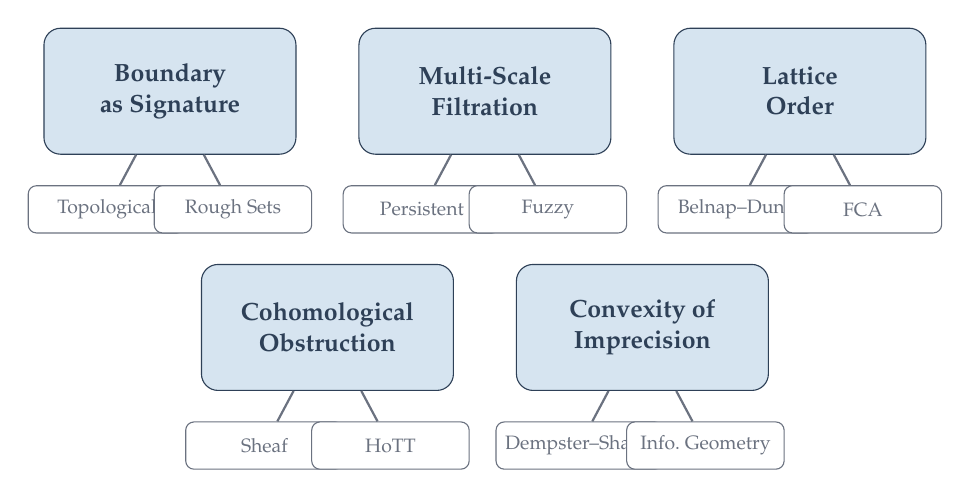
\begin{tikzpicture}[
    motif/.style={draw=accent, rounded corners=6pt, fill=softblue, minimum width=3.2cm, minimum height=1.6cm, align=center, font=\small\bfseries, text=accent},
    framework/.style={draw=midgray, rounded corners=3pt, fill=white, minimum width=2cm, minimum height=0.6cm, align=center, font=\scriptsize, text=midgray},
    arrow/.style={-{Stealth[length=5pt]}, thick, color=midgray}
]

% Motifs
\node[motif] (B) at (0,0) {Boundary\\as Signature};
\node[motif] (F) at (4,0) {Multi-Scale\\Filtration};
\node[motif] (L) at (8,0) {Lattice\\Order};
\node[motif] (O) at (2,-3) {Cohomological\\Obstruction};
\node[motif] (C) at (6,-3) {Convexity of\\Imprecision};

% Frameworks under each motif
\node[framework] (b1) at (-0.8,-1.5) {Topological};
\node[framework] (b2) at (0.8,-1.5) {Rough Sets};

\node[framework] (f1) at (3.2,-1.5) {Persistent};
\node[framework] (f2) at (4.8,-1.5) {Fuzzy};

\node[framework] (l1) at (7.2,-1.5) {Belnap--Dunn};
\node[framework] (l2) at (8.8,-1.5) {FCA};

\node[framework] (o1) at (1.2,-4.5) {Sheaf};
\node[framework] (o2) at (2.8,-4.5) {HoTT};

\node[framework] (c1) at (5.2,-4.5) {Dempster--Shafer};
\node[framework] (c2) at (6.8,-4.5) {Info.\ Geometry};

% Connecting lines
\draw[midgray, thick] (B) -- (b1);
\draw[midgray, thick] (B) -- (b2);
\draw[midgray, thick] (F) -- (f1);
\draw[midgray, thick] (F) -- (f2);
\draw[midgray, thick] (L) -- (l1);
\draw[midgray, thick] (L) -- (l2);
\draw[midgray, thick] (O) -- (o1);
\draw[midgray, thick] (O) -- (o2);
\draw[midgray, thick] (C) -- (c1);
\draw[midgray, thick] (C) -- (c2);

\end{tikzpicture}
\end{center}

\vspace{0.3cm}

Across the twelve frameworks, five structural motifs recur with striking consistency. These are not analogies or superficial similarities; they are genuine mathematical commonalities, suggesting that the geometry of unresolution has deep invariant structure.

\textbf{1. Boundary as Signature.} In topological epistemic logic, the boundary $\partial A$ is the zone of genuine ignorance---where the proposition is consistent with knowledge but not entailed. In rough set theory, the boundary region $\mathrm{BN}_R(X)$ is the zone where distinctions are insufficient to decide membership. In fuzzy topology, the boundary is the zone of intermediate membership value. In paraconsistent logic, the boundary is the zone where both $P$ and $\neg P$ have non-zero truth value. In every framework, unresolution \emph{lives on a boundary}---a lower-dimensional manifold separating regions of full resolution. The thickness, shape, and topology of this boundary are geometric invariants of the unresolved state.

\textbf{2. Multi-Scale Filtration.} Persistent homology explicitly parametrises analysis by a continuous parameter $\epsilon$ (distance threshold), revealing how topological features emerge and dissolve at different scales. This idea recurs throughout: rough set theory refines indiscernibility relations (each refinement is a finer scale); fuzzy topology thresholds membership values (each threshold is a scale); Dempster--Shafer theory can be conditioned by varying evidential strength (a filtration through layers of evidence); even category theory asks how structures exist at different levels of abstraction. Unresolution is \emph{always} scale-dependent, and the pattern of scale-dependence encodes crucial information about the nature of the irresolution.

\textbf{3. Lattice Order.} The bilattice of Belnap--Dunn, the concept lattice of FCA, the orthomodular lattice of quantum logic, and the poset of open sets in topological logic all provide partial orders on epistemic states. In each case, unresolution corresponds to incomparable elements---states that cannot be ordered by entailment or generality. The width of the lattice (the size of the maximum antichain) measures the ``degree of pluralism'' in the unresolved state: how many fundamentally different positions coexist? The height measures the depth of subsumption: how many levels of refinement are needed to go from maximal ignorance to maximal resolution?

\textbf{4. Cohomological Obstruction.} Sheaf cohomology detects the failure of local-to-global extension: local coherence cannot be glued into global coherence, and the non-zero cohomology class is an obstruction. HoTT detects higher identity structure that resists truncation: there are multiple non-compatible ways of identifying two concepts. Category theory detects the non-existence of limits: a diagram cannot be universally reconciled. In each case, unresolution is characterised as a \emph{cohomological or categorical obstruction}---an algebraic invariant that blocks a construction that would otherwise be possible. These obstructions are the deepest kind of unresolution: they cannot be eliminated by local adjustments.

\textbf{5. Convexity of Imprecision.} The credal sets of Dempster--Shafer theory form convex polytopes in the probability simplex. The set of probability distributions within a Fisher ball is convex. Rough set boundary regions, viewed as sets of possible classifications, form convex regions in appropriate senses. The space of fuzzy membership functions consistent with given constraints is convex. This is not accidental: unresolution is \emph{convex}---any ``mixture'' or ``interpolation'' of two ways of being unresolved is itself a way of being unresolved. This means unresolution has no internal gaps or holes: it is a connected, topologically simple region in the space of epistemic states. Convexity implies that there are well-defined extremal points (the most decisive conclusions available) and well-defined geometric measures (distances, diameters, volumes).

These five motifs are the skeleton of the geometry of unresolution. Any particular framework emphasises some motifs over others, but all five appear in every framework when examined closely.

\newpage

% ====================================================================
\section{Toward a Unified Hierarchy of Frameworks}
\label{sec:hierarchy}

The twelve frameworks are not independent theories of unresolution; they form a hierarchy connected by \emph{functorial relationships}---precise mathematical translations from one framework to another.

\begin{center}
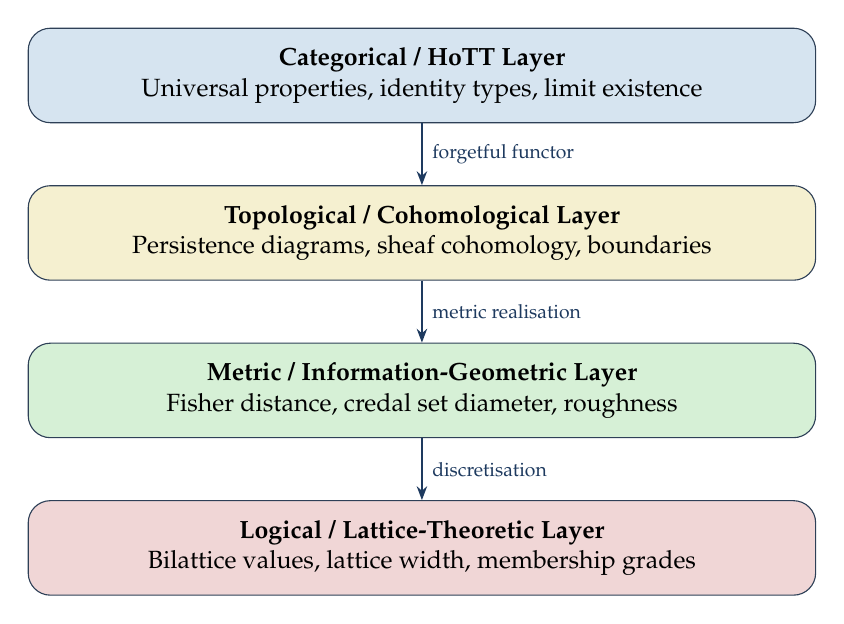
\begin{tikzpicture}[
    layer/.style={draw=accent, rounded corners=8pt, minimum width=10cm, minimum height=1.2cm, align=center, font=\small},
    larrow/.style={-{Stealth[length=5pt]}, thick, color=deepblue}
]

\node[layer, fill=softblue] (top) at (0,4) {\textbf{Categorical / HoTT Layer}\\ Universal properties, identity types, limit existence};
\node[layer, fill=softyellow] (mid) at (0,2) {\textbf{Topological / Cohomological Layer}\\ Persistence diagrams, sheaf cohomology, boundaries};
\node[layer, fill=softgreen] (low) at (0,0) {\textbf{Metric / Information-Geometric Layer}\\ Fisher distance, credal set diameter, roughness};
\node[layer, fill=softred] (base) at (0,-2) {\textbf{Logical / Lattice-Theoretic Layer}\\ Bilattice values, lattice width, membership grades};

\draw[larrow] (top) -- node[right, font=\scriptsize, text=deepblue] {forgetful functor} (mid);
\draw[larrow] (mid) -- node[right, font=\scriptsize, text=deepblue] {metric realisation} (low);
\draw[larrow] (low) -- node[right, font=\scriptsize, text=deepblue] {discretisation} (base);

\end{tikzpicture}
\end{center}

\subsubsection*{The Base Layer: Logical and Lattice-Theoretic}

At the most concrete level, logical frameworks (Belnap--Dunn, FCA, quantum logic, fuzzy sets) provide discrete or finitely-graded models of unresolution. They classify unresolution into \emph{types}:
\begin{itemize}
\item Ignorance ($\bot$) vs.\ contradiction ($\top$) in Belnap--Dunn.
\item Comparable vs.\ incomparable elements in FCA.
\item Distributive vs.\ non-distributive lattices in quantum logic.
\item Degree of membership in fuzzy sets.
\end{itemize}

These frameworks answer the question: \emph{What kind of unresolution is this?}

\subsubsection*{The Metric Layer: Information-Geometric and Probabilistic}

At the next level, information geometry and Dempster--Shafer theory equip the space of epistemic states with continuous measures---distances, volumes, diameters. They quantify unresolution:
\begin{itemize}
\item Fisher distance: how far is the current credal state from full resolution?
\item Credal set diameter: how much variability is there in the resolutions consistent with current evidence?
\item Dempster--Shafer belief-plausibility gap: how much evidence remains to be gathered?
\end{itemize}

These frameworks answer: \emph{How much unresolution is present?}

\subsubsection*{The Topological Layer: Persistent Homology and Sheaf Cohomology}

At a more abstract level, persistent homology, sheaf cohomology, and topological epistemic logic capture the \emph{shape} of unresolution:
\begin{itemize}
\item Persistence diagrams: at what scales does unresolution exist? Which scales are robust?
\item Sheaf cohomology: where (in which inter-topic boundaries) does global inconsistency arise?
\item Topological boundaries: what is the dimension and connectivity of the unresolved region?
\end{itemize}

These frameworks answer: \emph{What is the structure of unresolution?}

Topological invariants are stronger than metric invariants: if two systems are homeomorphic (topologically equivalent), their unresolution has the same shape even if the metric differs. Metric invariants can change while topological ones persist.

\subsubsection*{The Categorical Layer: Category Theory and HoTT}

At the most abstract level, category theory and HoTT provide the ultimate classification: they ask whether unresolution is resolvable \emph{in principle}, independent of the particular realisation:
\begin{itemize}
\item Limit existence: can the claims be universally reconciled? (In this category? In any category?)
\item Identity type h-level: in how many non-equivalent ways can the claims be identified?
\item Universal properties: what is the structural reason for unresolvability?
\end{itemize}

These frameworks answer: \emph{Is this unresolution fundamental or merely apparent?}

\subsubsection*{Connections Between Layers}

The transitions between layers are not arbitrary:

\textbf{Topological $\to$ Metric.} A topological space can be given a Riemannian metric (for example, the Fisher metric on the probability simplex). This ``realises'' the topology as a metric space. Information preserved: continuous functions become isometries or quasi-isometries; topological features are tracked by metric distances.

\textbf{Metric $\to$ Logical.} A metric space (with distance threshold $\epsilon$) can be ``discretised'': two states are equivalent if they are within distance $\epsilon$. This creates a partition of the space. Information preserved: metric relationships become ordering relationships; distances become ordering distances.

\textbf{Logical $\to$ Categorical.} A lattice or poset can be viewed as a category where morphisms are the order relationships. The universal properties of this category encode the combinatorial structure of the poset.

\subsubsection*{Multiple Realisations}

The same abstract structure can have multiple metric or topological realisations. For example:
\begin{itemize}
\item The same bilattice (Belnap--Dunn structure) can be equipped with different metric distances.
\item The same topological space can be equipped with different Riemannian metrics.
\item The same category can have different models.
\end{itemize}

This is an advantage: it means we can choose the realisation (metric, topology, category) that best fits our problem, while maintaining abstract structural properties across choices.

\newpage

% ====================================================================
\section{Computational Feasibility and Algorithmic Complexity}
\label{sec:computational}

For Noosphere and other epistemic systems, the practical question is: which frameworks can be computed efficiently on real-sized knowledge graphs?

\subsection{Complexity Summary}

\begin{center}
\begin{tabular}{|l|c|c|}
\hline
\textbf{Framework} & \textbf{Complexity} & \textbf{Feasible Scale} \\
\hline
Persistent Homology & $O(n^2 \log n)$ to $O(n^3)$ & $n \leq 50{,}000$ claims \\
Topological Epistemic Logic & NP-hard & $n \leq 100$ propositions \\
Sheaf Cohomology & $O(2^{|U|} \cdot n^3)$ & $|U| \leq 8$ topics \\
Rough Set Theory & $O(n \log n)$ per refinement & $n \leq 1{,}000{,}000$ objects \\
Formal Concept Analysis & NP-hard (lattice construction) & $n \leq 1000$ objects/attributes \\
Paraconsistent Logic & $O(n)$ (evaluation) & $n \leq 1{,}000{,}000$ clauses \\
Quantum Logic & $O(n^2)$ (Gram--Schmidt) & $n \leq 10{,}000$ subspaces \\
Dempster--Shafer & $O(2^{|\Theta|})$ exact & $|\Theta| \leq 20$ hypotheses \\
Information Geometry & $O(n^3)$ (interior-point LP) & $n \leq 1000$ parameters \\
Category Theory & Undecidable in general & Finite categories $\leq 100$ objects \\
Homotopy Type Theory & Decidable (type-checking) & Feasible for well-structured theories \\
Fuzzy Topology & $O(n \log n)$ & $n \leq 1{,}000{,}000$ elements \\
\hline
\end{tabular}
\end{center}

\subsection{Recommendations for Noosphere}

\textbf{Tier 1 (Fast, usable at scale):} Rough set theory, paraconsistent logic evaluation, fuzzy topology. These can handle large claim graphs and provide immediate feedback.

\textbf{Tier 2 (Moderate, usable on subgraphs):} Persistent homology (on embedded claim clusters), formal concept analysis (on individual topics). These should be recomputed periodically (e.g., hourly) on recent claims.

\textbf{Tier 3 (Slow, usable for deep analysis):} Sheaf cohomology, Dempster--Shafer (with approximations), information geometry. These should be reserved for focused investigation of particularly unresolved tensions.

\textbf{Tier 4 (Theoretical):} Category theory, HoTT. These can guide the design of Tier 1--3 tools but are not directly computable at scale.

\subsection{Approximation Strategies}

For frameworks that are too slow:
\begin{itemize}
\item \textbf{Dempster--Shafer with many hypotheses:} use Markov chain Monte Carlo to sample the belief and plausibility ranges.
\item \textbf{Sheaf cohomology with many topics:} use persistent cohomology (track cohomology changes as topics are added).
\item \textbf{FCA lattice construction:} use iterative lattice sampling or approximations like the iceberg lattice.
\item \textbf{Category limits:} check necessary conditions for limit existence (injectivity, commutativity) before attempting construction.
\end{itemize}

\newpage

% ====================================================================
\section{A Taxonomy of Unresolution}
\label{sec:taxonomy}

We now propose a unified classification of unresolution types, synthesising insights from all twelve frameworks.

\begin{center}
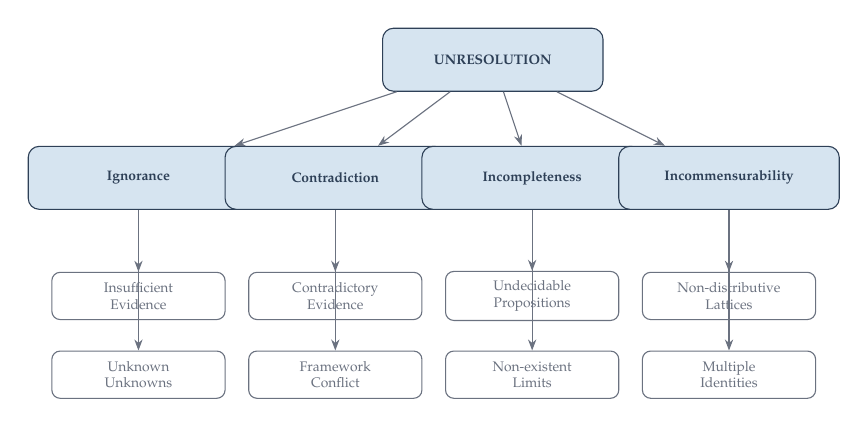
\begin{tikzpicture}[
    type/.style={draw=accent, rounded corners=4pt, fill=softblue, minimum width=2.8cm, minimum height=0.8cm, align=center, font=\tiny\bfseries, text=accent},
    subtype/.style={draw=midgray, rounded corners=3pt, fill=white, minimum width=2.2cm, minimum height=0.6cm, align=center, font=\tiny, text=midgray},
    arrow/.style={-{Stealth[length=4pt]}, color=midgray}
]

\node[type] (unres) at (5,6) {UNRESOLUTION};

\node[type] (ign) at (0.5,4.5) {Ignorance};
\node[type] (con) at (3,4.5) {Contradiction};
\node[type] (comp) at (5.5,4.5) {Incompleteness};
\node[type] (incom) at (8,4.5) {Incommensurability};

\node[subtype] (u1) at (0.5,3) {Insufficient\\Evidence};
\node[subtype] (u2) at (0.5,2) {Unknown\\Unknowns};

\node[subtype] (c1) at (3,3) {Contradictory\\Evidence};
\node[subtype] (c2) at (3,2) {Framework\\Conflict};

\node[subtype] (cmp1) at (5.5,3) {Undecidable\\Propositions};
\node[subtype] (cmp2) at (5.5,2) {Non-existent\\Limits};

\node[subtype] (ic1) at (8,3) {Non-distributive\\Lattices};
\node[subtype] (ic2) at (8,2) {Multiple\\Identities};

\draw[arrow] (unres) -- (ign);
\draw[arrow] (unres) -- (con);
\draw[arrow] (unres) -- (comp);
\draw[arrow] (unres) -- (incom);

\draw[arrow] (ign) -- (u1);
\draw[arrow] (ign) -- (u2);

\draw[arrow] (con) -- (c1);
\draw[arrow] (con) -- (c2);

\draw[arrow] (comp) -- (cmp1);
\draw[arrow] (comp) -- (cmp2);

\draw[arrow] (incom) -- (ic1);
\draw[arrow] (incom) -- (ic2);

\end{tikzpicture}
\end{center}

\subsection*{Type 1: Ignorance}

\textbf{Definition.} Unresolution due to lack of information or inability to distinguish between alternatives given current data.

\textbf{Characteristics.}
\begin{itemize}
\item Belnap--Dunn value: $\bot$ (neither true nor false).
\item Dempster--Shafer: large belief-plausibility gap.
\item Fisher distance: large (far from any resolved state).
\item Rough set roughness: high (many boundary objects).
\end{itemize}

\textbf{Subtypes.}
\begin{itemize}
\item \textbf{Insufficient evidence}: the relevant information simply hasn't been gathered. Examples: ``Will it rain tomorrow?'' (lacking a weather forecast); ``What is the true cause of X?'' (lacking experimental data).
  \emph{Response}: investigate, experiment, gather more data.

\item \textbf{Unknown unknowns}: the relevant dimensions of variation are unknown. Example: ``What do we not know about consciousness?'' The question itself lacks a frame.
  \emph{Response}: meta-investigation (investigate the space of possible investigations).
\end{itemize}

\subsection*{Type 2: Contradiction}

\textbf{Definition.} Unresolution due to the coexistence of mutually exclusive evidence or commitments.

\textbf{Characteristics.}
\begin{itemize}
\item Belnap--Dunn value: $\top$ (both true and false).
\item Paraconsistent logic: both $P$ and $\neg P$ are asserted.
\item Persistent homology: long-lived $H_1$ (cycles of contradiction).
\item Sheaf cohomology: non-zero $H^1$ (local-global inconsistency).
\end{itemize}

\textbf{Subtypes.}
\begin{itemize}
\item \textbf{Contradictory evidence}: different information sources point in opposite directions. Example: study A shows drug efficacy; study B shows inefficacy.
  \emph{Response}: meta-analysis, check for design differences, replicate.

\item \textbf{Framework conflict}: the contradiction arises from incompatible frameworks. Example: wave-particle duality; realism vs.\ idealism.
  \emph{Response}: recognize the frameworks are incommensurable, develop a larger framework incorporating both.
\end{itemize}

\subsection*{Type 3: Incompleteness}

\textbf{Definition.} Unresolution that cannot be eliminated within the current framework, even in principle.

\textbf{Characteristics.}
\begin{itemize}
\item Gödel incompleteness: true propositions that are unprovable.
\item Category theory: non-existent limits (diagrams that cannot be universally reconciled).
\item HoTT: identity type that is not contractible (multiple non-equivalent ways of identifying two concepts).
\end{itemize}

\textbf{Subtypes.}
\begin{itemize}
\item \textbf{Undecidable propositions}: formal statements that cannot be proven true or false within the system. Example: the continuum hypothesis in ZFC.
  \emph{Response}: accept the incompleteness; extend the framework with new axioms or move to a stronger system.

\item \textbf{Non-existent limits}: claims that cannot be universally reconciled within the current category.
  \emph{Response}: change the category (the ambient framework).
\end{itemize}

\subsection*{Type 4: Incommensurability}

\textbf{Definition.} Unresolution due to the claims operating within incompatible frameworks or using terms that have framework-dependent meanings.

\textbf{Characteristics.}
\begin{itemize}
\item Quantum logic: non-distributive lattice (some propositions lack independent truth values).
\item Topological epistemic logic: thick boundaries that do not shrink with evidence within the framework.
\item HoTT: identity type with non-trivial higher structure (multiple non-compatible ways of identifying claims).
\end{itemize}

\textbf{Subtypes.}
\begin{itemize}
\item \textbf{Non-distributive reasoning}: claims form an orthomodular lattice where context-dependence is irreducible. Example: position and momentum in quantum mechanics are not independently specifiable.
  \emph{Response}: embrace the complementarity; use the non-distributive lattice as the model.

\item \textbf{Multiple identities}: claims can be identified in multiple non-equivalent ways. Example: light as wave and light as particle are both valid but incompatible identifications.
  \emph{Response}: track the higher structure; represent claims as having a nontrivial identity type.
\end{itemize}

\begin{center}
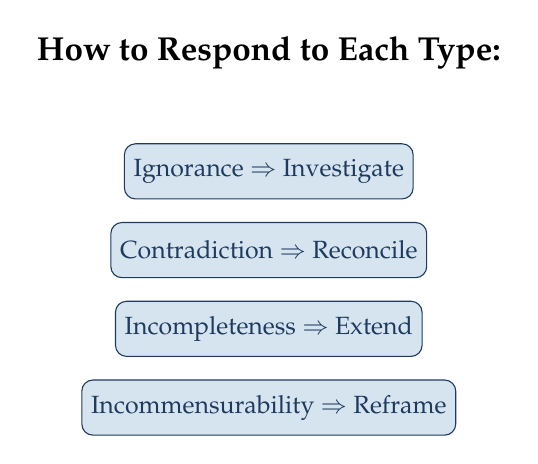
\begin{tikzpicture}[
    response/.style={draw=deepblue, rounded corners=4pt, fill=softblue, minimum width=3cm, minimum height=0.7cm, align=center, font=\small, text=deepblue},
    example/.style={draw=amber, rounded corners=3pt, fill=lightyellow, minimum width=2.5cm, minimum height=0.5cm, align=center, font=\footnotesize, text=amber}
]

\node at (0, 5) {\textbf{\large How to Respond to Each Type:}};

\node[response] (r1) at (0, 3.5) {Ignorance $\Rightarrow$ Investigate};
\node[response] (r2) at (0, 2.5) {Contradiction $\Rightarrow$ Reconcile};
\node[response] (r3) at (0, 1.5) {Incompleteness $\Rightarrow$ Extend};
\node[response] (r4) at (0, 0.5) {Incommensurability $\Rightarrow$ Reframe};

\end{tikzpicture}
\end{center}

\newpage

% ====================================================================
\section{Limitations and Open Problems}
\label{sec:limitations}

The twelve frameworks we've surveyed are powerful, but they have important limitations.

\subsection{What These Frameworks Cannot Do}

\textbf{1. They do not adjudicate between frameworks.} Category theory tells you that a diagram has no limit in category $\mathcal{C}$, but cannot tell you whether to move to a larger category or to abandon the ambition for a universal reconciliation. The choice is value-laden and depends on what you care about.

\textbf{2. They do not explain why unresolution arises.} Sheaf cohomology detects where global consistency fails, but does not tell you why---what the underlying reasons are. It diagnoses but does not explain the etiology.

\textbf{3. They assume well-structured inputs.} All frameworks assume claims can be meaningfully embedded in spaces, ordered in lattices, etc. But in practice, claims are messy: they have ambiguous scopes, context-dependent meanings, and vague boundaries. Preprocessing claims into mathematical objects requires judgment calls.

\textbf{4. They are coarse relative to the richness of real disagreement.} Two scholars can both hold consistent positions yet have deep disagreements about methodology, values, and interpretation. The frameworks detect disagreement but miss its texture.

\textbf{5. They do not prescribe action.} Knowing that a question is Gödel-undecidable or that a limit does not exist does not tell you what to \emph{do}. It tells you what is not possible in principle, but action requires value judgments.

\subsection{Open Problems}

\textbf{1. Integration of frameworks.} We've shown that twelve frameworks share common motifs, but we have not constructed a single grand framework that subsumes all twelve. What would such a framework look like? Is it even possible?

\textbf{2. Dynamical systems and evolution.} The frameworks are static: they describe unresolution at a moment in time. But real epistemic systems evolve: claims are added, refined, abandoned. How does unresolution evolve? Which dynamics lead to resolution vs.\ crystallization?

\textbf{3. Multi-agent unresolution.} Unresolution exists within a single agent's beliefs (this paper), but also between agents who disagree. How do the frameworks extend to multi-agent systems? When agents have different lattices or different categories, what is the geometry of their disagreement?

\textbf{4. Computational enhancements.} Most frameworks are NP-hard or worse. Can approximation algorithms or heuristics capture the essential geometry? Can machine learning be used to detect these structures in raw text or discourse?

\textbf{5. Validation.} We have not empirically validated these frameworks on real knowledge graphs or discourse. Do they actually help humans understand and resolve disagreement? We have theoretical justification but lacking empirical grounding.

\textbf{6. The geometry of resolution.} This paper focuses on the geometry of \emph{unresolution}, but what about the process of \emph{resolution}? If unresolution has structure, does resolution? What is the geometry of moving from one resolution to another?

\textbf{7. Consciousness and subjectivity.} All frameworks treat epistemology objectively: claims and their relationships. But understanding requires a knower, a perspective. How do these frameworks change when we consider the role of the epistemic agent?

\newpage

% ====================================================================
\section{Implications for the Noosphere Engine}
\label{sec:noosphere}

The Noosphere coherence engine is designed to maintain a graph of epistemic claims, track their consistency, and guide synthesis. The frameworks in this paper suggest concrete enhancements.

\subsection{Persistent Homology on Claim Embeddings}

\textbf{Algorithm Sketch.}

\begin{enumerate}
\item For $\epsilon$ from $\epsilon_{\min}$ to $\epsilon_{\max}$ in steps of $0.01$:
   \begin{itemize}
   \item Build Vietoris--Rips complex $K_\epsilon$: add 0-cells for claims and $k$-cells for all subsets of $k+1$ claims within $\epsilon$ distance.
   \item Compute homology $H_k(K_\epsilon)$ for $k = 0, 1, 2$.
   \item Track births and deaths of generators.
   \end{itemize}
\item Output: points (birth, death) in each persistence diagram.
\item Post-processing: for each long-lived feature with death $-$ birth $> $ threshold, identify the claims involved and mark as a structural tension.
\end{enumerate}

\textbf{Practical Use.}
\begin{itemize}
\item Run this weekly on recent claim clusters.
\item Display persistence diagrams in Noosphere UI: let users filter by lifetime.
\item Flag long-lived $H_1$ features as ``stubborn tensions'' worth investigating.
\item Track how persistence diagrams evolve: a feature that persists across weeks is structurally robust.
\end{itemize}

\subsection{Sheaf-Theoretic Consistency Checking}

\textbf{Algorithm Sketch.}

\begin{enumerate}
\item For each topic $U_i$: compute the set of locally coherent interpretations $I_i$ using an SMT solver or constraint satisfaction algorithm. Set $I_i = \{\text{interpretations consistent with all claims in } U_i\}$.
\item For each pairwise overlap $U_i \cap U_j$: check compatibility by computing $I_i|_{U_i \cap U_j} \cap I_j|_{U_i \cap U_j}$. If empty, record as a 1-cocycle.
\item Compute coboundary maps $\delta: C^0 \to C^1$ (changes in local interpretations that explain inconsistencies).
\item Compute $H^1 = \ker(\delta) / \mathrm{im}(\delta)$.
\item Output: non-zero cohomology classes (obstructions to global consistency).
\end{enumerate}

\textbf{Practical Use.}
\begin{itemize}
\item Run monthly on the full claim graph after major discussions.
\item Non-zero $H^1$ indicates that no local fix will resolve inter-topic tensions.
\item Use the cohomology class to identify which topic pairs have deepest conflict.
\item Guide the synthesis engine toward the most productive synthesis targets.
\end{itemize}

\subsection{Four-Valued Annotation}

\textbf{Enhancement to Coherence Assessment.}

Instead of binary ``coherent / incoherent'', annotate each claim with a Belnap--Dunn value:
\begin{itemize}
\item $\mathbf{t}$: strongly supported by evidence, no contrary evidence.
\item $\mathbf{f}$: strongly contradicted, no supporting evidence.
\item $\top$: contradictory evidence (some sources support, others contradict).
\item $\bot$: insufficient evidence to evaluate (hasn't been investigated).
\end{itemize}

\textbf{Decision Logic.}
\begin{itemize}
\item $\mathbf{t}$ or $\mathbf{f}$: claim is \emph{resolved}. No further investigation needed (unless new evidence emerges).
\item $\bot$: claim is \emph{ignorant}. Prioritize for investigation.
\item $\top$: claim is \emph{conflicted}. Do not investigate further within current framework; initiate conceptual revision discussion.
\end{itemize}

\textbf{Implementation.}

In Noosphere's coherence engine, compute:
\[
\text{annotation}(c) = \begin{cases}
\mathbf{t} & \text{if } P(\text{evidence supports } c) > 0.8 \text{ and } P(\text{evidence contradicts } c) < 0.1 \\
\mathbf{f} & \text{if } P(\text{evidence contradicts } c) > 0.8 \text{ and } P(\text{evidence supports } c) < 0.1 \\
\top & \text{if both probabilities are $> 0.3$} \\
\bot & \text{if both probabilities are $< 0.3$}
\end{cases}
\]

\subsection{Fisher Distance to Resolution}

\textbf{For Claims with Probability Estimates.}

For each claim $c$ with associated probability estimate $p_c$ and a credal set $S_c$ (the set of probabilities consistent with current evidence):

\begin{enumerate}
\item Compute the Fisher--Rao distance from the center of $S_c$ to each vertex of the probability simplex (fully resolved states $p = 0$ and $p = 1$).
\item Report the minimum distance as ``statistical distance to resolution.''
\item Track how this distance shrinks as new evidence is gathered.
\end{enumerate}

\textbf{Interpretation.}
\begin{itemize}
\item Distance $< 1$ standard evidence unit: question is nearly resolved.
\item Distance $1$--$10$: moderate unresolution.
\item Distance $> 10$: severe unresolution, unlikely to resolve with current methods.
\end{itemize}

\subsection{Rough Set Boundary Tracking}

\textbf{Refinement of Indiscernibility Relations.}

As Noosphere accumulates discussions and distinctions:
\begin{enumerate}
\item Maintain an indiscernibility relation $R$ on claims (which claims are indistinguishable given current information).
\item For each claim $c$, compute the roughness $\rho(c)$ with respect to $R$.
\item When new distinctions are proposed (new topics, new dimensions of evaluation):
   \begin{enumerate}
   \item Refine $R$ to $R'$ (finer equivalence classes).
   \item Recompute roughness $\rho'(c)$.
   \item Track the \emph{rate} of boundary shrinkage: $\Delta \rho = \rho - \rho'$.
   \end{enumerate}
\end{enumerate}

\textbf{Interpretation.}
\begin{itemize}
\item Fast shrinkage: the topic is epistemically tractable; continue with current approach.
\item Slow shrinkage: the topic is difficult; may require new conceptual foundations.
\item Plateau (shrinkage stops): the indistinguishability relation cannot be further refined; new measurement modalities needed.
\end{itemize}

\subsection{Dashboard Metrics}

A Noosphere dashboard could display:

\begin{center}
\begin{tabular}{|l|l|l|}
\hline
\textbf{Metric} & \textbf{Computation} & \textbf{Interpretation} \\
\hline
Topological Robustness & Persistence of $H_1$ features & Structural coherence across scales \\
Cohomological Obstruction & Dimension of $H^1$ & Irreducible inter-topic tensions \\
Bilattice Distribution & Histogram of $\{\mathbf{t}, \mathbf{f}, \top, \bot\}$ & Resolution breakdown \\
Fisher Distance & Median of min-distance-to-vertex & Overall closeness to resolution \\
Boundary Shrinkage & $\Delta \rho$ per discussion & Epistemic progress \\
Concept Lattice Width & Max antichain in FCA lattice & Conceptual diversity \\
\hline
\end{tabular}
\end{center}

\newpage

% ====================================================================
\section{Decision Flowchart: Which Framework to Use}
\label{sec:decision}

\begin{center}
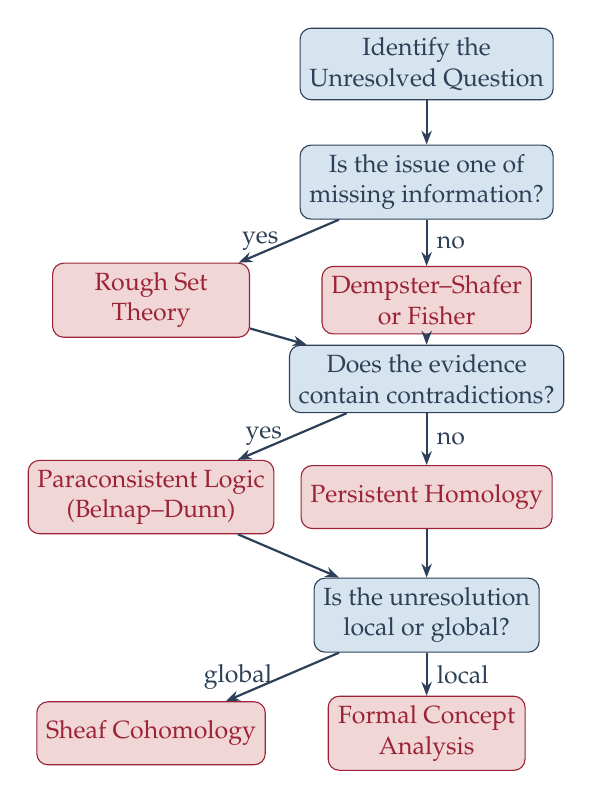
\begin{tikzpicture}[
    decision/.style={draw=accent, rounded corners=4pt, fill=softblue, minimum width=2.5cm, minimum height=0.8cm, align=center, font=\small, text=accent},
    outcome/.style={draw=deepred, rounded corners=4pt, fill=softred, minimum width=2.5cm, minimum height=0.8cm, align=center, font=\small, text=deepred},
    arrow/.style={-{Stealth[length=5pt]}, thick, color=accent}
]

\node[decision] (start) at (5, 10) {Identify the\\Unresolved Question};

\node[decision] (q1) at (5, 8.5) {Is the issue one of\\missing information?};
\node[outcome] (a1) at (1.5, 7) {Rough Set\\Theory};
\node[outcome] (a2) at (5, 7) {Dempster--Shafer\\or Fisher};

\node[decision] (q2) at (5, 6) {Does the evidence\\contain contradictions?};
\node[outcome] (a3) at (1.5, 4.5) {Paraconsistent Logic\\(Belnap--Dunn)};
\node[outcome] (a4) at (5, 4.5) {Persistent Homology};

\node[decision] (q3) at (5, 3) {Is the unresolution\\local or global?};
\node[outcome] (a5) at (1.5, 1.5) {Sheaf Cohomology};
\node[outcome] (a6) at (5, 1.5) {Formal Concept\\Analysis};

\draw[arrow] (start) -- (q1);
\draw[arrow] (q1) -- node[left, font=\small] {yes} (a1);
\draw[arrow] (q1) -- node[right, font=\small] {no} (a2);

\draw[arrow] (a1) -- (q2);
\draw[arrow] (a2) -- (q2);

\draw[arrow] (q2) -- node[left, font=\small] {yes} (a3);
\draw[arrow] (q2) -- node[right, font=\small] {no} (a4);

\draw[arrow] (a3) -- (q3);
\draw[arrow] (a4) -- (q3);

\draw[arrow] (q3) -- node[left, font=\small] {global} (a5);
\draw[arrow] (q3) -- node[right, font=\small] {local} (a6);

\end{tikzpicture}
\end{center}

\textbf{Flowchart Guide:}

\begin{enumerate}
\item \textbf{Start}: You've identified a piece of unresolved knowledge. What kind is it?

\item \textbf{Question 1: Missing information?}
   \begin{itemize}
   \item \textbf{Yes}: Use \textbf{Rough Set Theory} (Section~\ref{sec:algebraic}) to measure how much information is missing and what new distinctions are needed.
      Or use \textbf{Dempster--Shafer} or \textbf{Fisher Information} (Section~\ref{sec:probabilistic}) to quantify the magnitude of uncertainty.
   \item \textbf{No}: The information you have is contradictory or incommensurable. Proceed to Question 2.
   \end{itemize}

\item \textbf{Question 2: Contradictory evidence?}
   \begin{itemize}
   \item \textbf{Yes}: Use \textbf{Paraconsistent Logic} (Section~\ref{sec:paraconsistent}) to distinguish genuine contradiction ($\top$) from ignorance ($\bot$). Then decide whether to investigate further or revise frameworks.
   \item \textbf{No}: The unresolution is deeper---claims are framework-dependent or incommensurable. Use \textbf{Persistent Homology} (Section~\ref{sec:persistent}) to find which tensions persist across scales.
   \end{itemize}

\item \textbf{Question 3: Where is the unresolution?}
   \begin{itemize}
   \item \textbf{Global (across multiple topics):} Use \textbf{Sheaf Cohomology} (Section~\ref{sec:sheaf}) to locate which inter-topic boundaries carry the deepest tension.
   \item \textbf{Local (within a single topic):} Use \textbf{Formal Concept Analysis} (Section~\ref{sec:fca}) to reveal incompatible ways of organizing the concepts in that topic.
   \end{itemize}

\end{enumerate}

\newpage

% ====================================================================
\section{Conclusion}
\label{sec:conclusion}

We have surveyed twelve mathematical frameworks---topological, algebraic, logical, probabilistic, and categorical---that characterise unresolution not as formless ignorance but as a structured geometric phenomenon. The central findings are:

\subsection*{Structural Findings}

\textbf{1. Unresolution is geometrically structured.} It is not homogeneous darkness but a landscape with features: boundaries, scales, obstructions, types. Each feature carries information about the \emph{why} of unresolution and the \emph{what} of resolution.

\textbf{2. Five motifs recur across all frameworks.} Boundary as signature, multi-scale filtration, lattice order, cohomological obstruction, and convexity of imprecision appear in every framework when examined closely. These are the skeleton of the geometry of unresolution.

\textbf{3. The frameworks form a hierarchy.} They are not independent theories but related by functorial maps, forming a tower of increasing abstraction: logical $\to$ metric $\to$ topological $\to$ categorical.

\textbf{4. Unresolution is scale-dependent.} A tension that is catastrophic at one scale may dissolve at another. Persistent homology makes this quantitative and computable.

\textbf{5. Local consistency does not guarantee global consistency.} Sheaf cohomology reveals that claims can be individually coherent yet globally incoherent. This is not a defect in reasoning but a structural feature of any system with multiple topics.

\textbf{6. Some unresolution is irreducible.} Gödel incompleteness, categorical limits that do not exist, identity types with non-trivial higher structure---these reveal unresolution that cannot be eliminated by investigation or refinement within the current framework. Recognising irreducible unresolution is as important as resolving the reducible kind.

\subsection*{Practical Implications}

For Noosphere and similar epistemic systems:

\begin{itemize}
\item \textbf{Diagnose, don't just detect.} Instead of flagging unresolution as a system error, diagnose its \emph{type}: Is it ignorance, contradiction, incompleteness, or incommensurability? The response differs.

\item \textbf{Prioritise by robustness.} Long-lived topological features matter more than ephemeral ones. Concentrate effort on tensions that persist across scales and topics.

\item \textbf{Distinguish local from global.} Not every local tension requires global reconciliation. Use sheaf cohomology to find where global inconsistency actually arises.

\item \textbf{Measure distance to resolution.} Fisher information gives a metric on the space of epistemic states. Know how far you are from resolution in statistical space.

\item \textbf{Accept irreducible unresolution.} Some tensions will not resolve. When you detect categorical non-existence of limits or Gödelian undecidability, stop trying to resolve and start reconceptualising.
\end{itemize}

\subsection*{Philosophical Implications}

\textbf{On the nature of knowledge:} Knowledge is not binary (known or unknown) but richly structured. The geometry of unresolution reveals what is being sought, what obstacles stand in the way, and which approaches are productive.

\textbf{On disagreement:} When intelligent people disagree, it is not always due to irrationality or bad faith. Often it reflects genuine structural tensions in the problem space itself. Recognising the geometry of unresolution transforms conflict from a failure into an opportunity to understand the deep structure of the question.

\textbf{On the limits of inquiry:} Some questions cannot be resolved through more investigation because the unresolution is not epistemic but structural. The frameworks reveal which kind of unresolution you're dealing with.

\subsection*{On Noosphere's Purpose}

Theseus's Noosphere engine is designed to track the evolution of ideas and find the deep structure beneath surface-level discourse. The geometry of unresolution is exactly this deep structure. It is not merely a theoretical curiosity; it is the operational machinery of an epistemic system that aims to be coherent and truthful.

As claims accumulate and discussions deepen, unresolution will emerge. When it does, Noosphere should not collapse into a binary choice (resolve or abandon). Instead, it should use the tools in this paper to understand the unresolution: its type, its location, its robustness, its depth. Some unresolutions will dissolve under scrutiny. Others will reveal deep structural insights. Still others will prove irreducible, requiring a shift in framework.

In all cases, the geometry of unresolution is not a problem to be solved but a compass pointing toward deeper understanding.

\vspace{1cm}
\begin{center}
\rule{3cm}{0.4pt}
\end{center}

\appendix

\section{Further Reading}

\textbf{Persistent Homology:}
Carlsson, G. (2009). ``Topology and data.'' \textit{Bulletin of the American Mathematical Society}, 46(2), 255--308.

\textbf{Sheaf Theory and Cohomology:}
Bredon, G. E. (1997). \textit{Sheaf Theory} (2nd ed.). Springer.

\textbf{Rough Sets:}
Pawlak, Z. (1991). \textit{Rough Sets: Theoretical Aspects of Reasoning about Data}. Kluwer.

\textbf{Formal Concept Analysis:}
Ganter, B., \& Wille, R. (1999). \textit{Formal Concept Analysis: Mathematical Foundations}. Springer.

\textbf{Paraconsistent Logic:}
Priest, G. (2002). \textit{Beyond the Limits of Thought} (2nd ed.). Oxford University Press.

\textbf{Dempster--Shafer Theory:}
Shafer, G. (1976). \textit{A Mathematical Theory of Evidence}. Princeton University Press.

\textbf{Information Geometry:}
Amari, S. (2016). \textit{Information Geometry and Its Applications}. Springer.

\textbf{Homotopy Type Theory:}
The Univalent Foundations Program. (2013). \textit{Homotopy Type Theory: Univalent Foundations of Mathematics}. \url{https://homotopytypetheory.org}.

\vspace{0.5cm}

\end{document}
